% Created 2015-08-17 Mon 22:19
\documentclass[9pt,b5paper]{article}
\usepackage{graphicx}
\usepackage{xcolor}
\usepackage{xeCJK}
\setCJKmainfont{SimSun}
\usepackage{longtable}
\usepackage{float}
\usepackage{textcomp}
\usepackage{geometry}
\geometry{left=0cm,right=0cm,top=0cm,bottom=0cm}
\usepackage{multirow}
\usepackage{multicol}
\usepackage{listings}
\usepackage{algorithm}
\usepackage{algorithmic}
\usepackage{latexsym}
\usepackage{natbib}
\usepackage{fancyhdr}
\usepackage[xetex,colorlinks=true,CJKbookmarks=true,linkcolor=blue,urlcolor=blue,menucolor=blue]{hyperref}


\lstset{language=c++,numbers=left,numberstyle=\tiny,basicstyle=\ttfamily\small,tabsize=4,frame=none,escapeinside=``,extendedchars=false,keywordstyle=\color{blue!70},commentstyle=\color{red!55!green!55!blue!55!},rulesepcolor=\color{red!20!green!20!blue!20!}}
\author{deepwaterooo}
\date{\today}
\title{The autobiography of deepwaterooo\textasciitilde{} \linebreak Outline \& Reader's Guide}
\hypersetup{
  pdfkeywords={},
  pdfsubject={},
  pdfcreator={Emacs 24.3.1 (Org mode 8.2.7c)}}
\begin{document}

\maketitle
\tableofcontents


\section{initial\ldots{}}
\label{sec-1}
Search "\textbf{deepwaterooo}" from \textbf{mitbbs.com}, you will find tons of posts, yes, that's me\textasciitilde{}
\subsection{Autobiography contents}
\label{sec-1-1}
\begin{itemize}
\item \textbf{part 1:} all my 33 years life before Aug 2012, in which year, I continued with a computer science master's degree;
\item \textbf{part 2:} computer science master's degree first three semesters record up to hw4 of \textbf{compiler design};
\item \textbf{part 3:} finish recording compiler design hws related, included 4th semester, record up to summer 2014;
\item \textbf{part 4:} record the last year's suffering, which greatly affected my character ever since mid Nov, 2014\ldots{}.
\end{itemize}
\subsection{other notes}
\label{sec-1-2}
\begin{itemize}
\item will write more and \textbf{add English Notes when necessary}.
\item \textbf{Law} related documents will be uploaded later.
\item will organize outline later for reader's convenience, and also to make a point.
\end{itemize}

\section{partial outline: County}
\label{sec-2}
\subsection{My life has been so much \textbf{tortured} here by the department minority and local county:}
\label{sec-2-1}
\begin{itemize}
\item The ex-advisor and the famous professor from the department kept me staying here for MS CS by giving me permission to select more credits than 7, which is the credits they allow for first semester student;
\item The ex-advisor tried to produce a love affair gossip between him and me;
\begin{itemize}
\item \textbf{part 2}, Chapter 45, \textbf{page 197 - 199}
\item He asked me to walk together with him on campus more than twice.
\item He touched my hand once;
\item he automatically changed his contact email address from university email to gmail accounts, insisted me to use his gmail account to contact him, tried to reply one email only to me instead of all other classmates, but got looked down by me because of his bad work performance for at least once;
\item A university 19 years old girl was gun-shot by a my current university professor because the girl wanted to end their love-relationship but he doesn't want to. When the girl reported to the university, he got fired, and then he killed both the girl and himself in \textbf{Aug 2011};
\item \url{https://github.com/deepwaterooo/AndroidAppProgramming} updated 12/19/2014, Friday, mentioned this fact half a year ago;
\item \url{https://github.com/deepwaterooo/SeniorDesign}
\end{itemize}
\end{itemize}
\subsection{Who tortured/wasted my more than one and half years life between 3/7/2013 and 2/27/2015?}
\label{sec-2-2}
\begin{itemize}
\item My cousin set permanent protection order against me under local police/country judge's pressure.
\item I was told wrong information by ex-layer that my 3/7/2013 court case would expire in one-year (which means expire on 3/7/2014);
\item I was blocked from learning the information about the permanent protection order they set against me.
\begin{itemize}
\item During Jan-Mar 2013 court season, I only got information about temporary protection order, attended 1/31/2013 court, but they didn't give me any result information.
\item I first heard about this piece of information on 12/27/2014. I have been waiting for one thing only. Who tortured/wasted my more than one and half years life between 3/7/2013 and 2/27/2015?
\item The permanent protection order was finally served on me on 2/27/2015, and the \textbf{permanent protection order} expires on \textbf{3/21/2017};
\end{itemize}
\end{itemize}

\section{partial outline: University}
\label{sec-3}
\subsection{Facts}
\label{sec-3-1}
\begin{itemize}
\item Ex-advisor and the famous professor from the program and department made me stay for MS. CS by giving me permission for selecting more credits rather than they planned 7 credits.
\item (Fall 13:) The compiler design course instructor made the course contents especially hard only for the propose of ruining my professional reputation which was built during the summer after I have accomplished all my projects successfully.
\item (Spring 14:) During Fall 12, when cs121 couse instructor who has only master's degree, and cs210 programming language course instructor \textbf{both didn't cover Object-oriented programming topics}, I had been throw into fire by cs572 EC for OO programming, function pointers etc (EC project 1, \textbf{part 3}, Chapter 24, \textbf{page 183-184}). EC projects just like AI projects, were heavily programming-concentrated, I finished most projects successfully with the \textbf{best methods} especially for \textbf{project 1 and project 2}. Because I have new focus between 3/25-4/30/2014 (and some early May days as well) for algorithms practise (problems solved can be found at \url{https://github.com/deepwaterooo/MyAlgorithms/tree/master/LeetCode_c\%2B\%2B_0325-04302014-100} ), my project 3 code has shortcomings. I understand all the theory, and for the EC course, the instructor requires only the final report, he always doesn't require codes, even my AI \textbf{Decision Tree} codes (project can be found at \url{https://github.com/deepwaterooo/csMajorCourses-Projects/tree/master/cs570AI_Project4_DecisionTrees}), which project I was the \textbf{only one} student who dare to and took all the effort to work on this project for couple of years.
\item (Fall 14:) My advisor tried to block me from selecting Statistics related courses ever since Fall 13 (emails can be found at \textbf{part 2}, Chapter 12, \textbf{page 97-98}). This semester the department doesn't offer any Statistics-related course for us at all. I selected \textbf{cs480 Senior Design}, with five to six course instructor in total, with wired \textbf{Team Contract} requirements, but still, I got kicked out from the team by the department on propose, because they don't want to give me any opportunity for coming spring semester \textbf{cs481}, which was reqiured when I registered cs480.
\item (Fall 14:) The Andriod App Programming instructor was so \textbf{unfair} towards me and especially mean by saying that I need more \textbf{practice} on propose because I would NOT have any practice time (OPT). I do need more practise but the university gave me no opportunities for practise at all. He is the representative of this \textbf{dark and mean} culture.
\item (Spring 15:) The department successfully blocked me from getting a TA for any more professional practise, required and got my student office one seat back in Nov 2014 as well, leaving me no good study environment at all. They claimed that because I was NOT a TA any more, so I have no student office seat, and have no entrance to the department during evening/nights and weekend. From 08/12-1/14, for 3 semesters I don't have TA as well, why they gave me a seat before? And I had always been using the seat for study. What changed? The culture changed. No, it's not change, just the \textbf{dark and mean} culture becomes more obvious, that's all!
\item (Spring 15:) While I have to stuggle every step out for my graduate project with barely any constructive help from the advisor, I have to do labor work in campus food court to make a living. As the youngest child in my family and having always been a student, I sware this is the hardest labor work for me ever! And I have to do that most hard work in the food court as well! What's \textbf{mean}, treat international student this way is mean! I have to walk miles in total to collect all the stuff needed for salad bar for each evening when I have shifts.
\item I only got As from course when I upload all the homework and progress into github, which happened from last semester. As a smart and extraordinary student who can finish a tic-tac-toe especially difficult project within the first month of my new major, how come my professional progress were so slow back in school? The reason is simple, they tried every mean ways to block a international student from achieving sucess!
\end{itemize}
\subsection{Conclusion}
\label{sec-3-2}
\begin{itemize}
\item And what really \textbf{mean to death} is that, when a student could potentially get an work opportunity from industry, the department and university tried and blocked me twice from getting it! 
\begin{itemize}
\item I had been kind and try to understand and tolerant all the difficulties here. I had tried to be kind and understand somebody else's difficulties, but up to this point, I would have to say:
\item Some instructor's gene should be extinguished from the universe so he would NOT be able to torture somebody else's life. So he DESERVE having NO child;
\item Some instructor DESERVEs to have children with inherited diseases, so he could potentially try to understand somebody else's difficulties;
\item Some instructor DESERVEs to have his reputation ruined, because he plays mean and dark, just like he could found his nephew \$5000 for barely any project research.
\item I know there is a song called "God bless American". I would have to say may God bless all the jerks go to hell\textasciitilde{} When they were about to die, may God remind them to remember that years ago there was a international student blessed them all go to hell\textasciitilde{}
\end{itemize}
\item This is \textbf{www.github.com}. What I have suffered here from the university should be broadcasted world wide. I will maintain this deepwaterooo account \textbf{\url{https://github.com/deepwaterooo}} at least for yeas so that Chinese community would never come this chicken universities like my current one, and also so that international students would be able to carefully consider if they really need to studyin chicken universities like this!
\end{itemize}

\section{Ph.D? Go to hell\textasciitilde{}!}
\label{sec-4}
\subsection{about Ph.D}
\label{sec-4-1}
\begin{itemize}
\item \textbf{Part 4}, Chapter 42, \textbf{page 131-132}, Ph.D? Go to hell\textasciitilde{}!
\begin{itemize}
\item Not anybody can continue with a Ph.D at whatever age. Ask me to continue with a Ph.D at current age? Go to hell\textasciitilde{}!
\item When they asked me to stay with a master three years ago, have they ever mentioned anything about I will have to continue with a Ph.D?
\item I hate people torture my life this way, and hate they so much, they all DESERVE go to hell!
\end{itemize}
\end{itemize}
\subsection{about Law-related Documents}
\label{sec-4-2}
\begin{itemize}
\item will upload and update them later when I get all the things on hand done.
\end{itemize}

\section{Study Plan \& Degree Audit}
\label{sec-5}
\begin{itemize}
\item About study plan, previous processes can be traced at \url{https://github.com/deepwaterooo/midiController}
\item After four round of modification, after another one week of waiting, the one course of unnecessary was finally removed up to today at 13:09, but the other one course cs449 which I removed and got all approved by the advisor/department/graduate school IS still listed on study plan.
\item Quote from degree audit: "Notes: May 15 2015 remove CS 449 and CS XXX. ADD CS 520 and CS 480"
\item This is going to be a NEVER-ENDING process! what the XXXX
\end{itemize}

\section{about graduation}
\label{sec-6}
I mean to paste all the necessary emails here with critical information (like name, email address etc) hiden, but apparently after graduation, I was not careful enough to keep the password changed every 3 or 4 months, and I lost access into my university email. The only drafts/leftovers were those when I reply emails, felt I need write in emacas local in my laptop, so several emails are pasted below. 
\subsection{Will you be graduating this summer?}
\label{sec-6-1}
(graduate personnel) (cheric@uxxxx.edu)
Sent:        Thursday, June 18, 2015 8:50 AM
To:        (graduate personnel) ((graduate personnel)@uxxxx.edu)

Hi,

You are receiving this email because you have an active application to graduate this summer. We would like to keep our records as current as possible, so  would you please let me know if you are pretty confident you will graduate this summer, or if I should cancel your summer application, so you can re apply for a different semester.

When you reply, please include your first and last name in the email. And I need to hear back from you by Friday, June 26, please.

Thank you! And I hope your summer is going well!

graduate personnel
College of Graduate Studies

\subsection{Hi (graduate personnel),}
\label{sec-6-2}

Yes I did apply for graduation before the end of spring semester. I had thought that I have finished all the necessary steps and will for sure graduate this August, so when I received this email, I was surprised. 

I had thought that I would be able to enjoy working in industry for couple of years with peace in mind, but I have not been able to find any industry working opportunity. Since I was NOT able to work in industry and not able to enjoy the work which I like the most, at the age of 36, why not enjoy life then? Instead of pursuing any Doctor's degree, I would rather try to have a baby before it's too late, especially when I have significant physically syndromes diagnosed already.  

So, YES, I am pretty confident that I will graduate this summer. So please you don't need to cancel my summer application, and I don't need any different semester. 

First Name: (me\textasciitilde{}~\textasciitilde{}) 
Last Name: (me\textasciitilde{}~\textasciitilde{}) 

thanks,
(me\textasciitilde{}~\textasciitilde{}) 

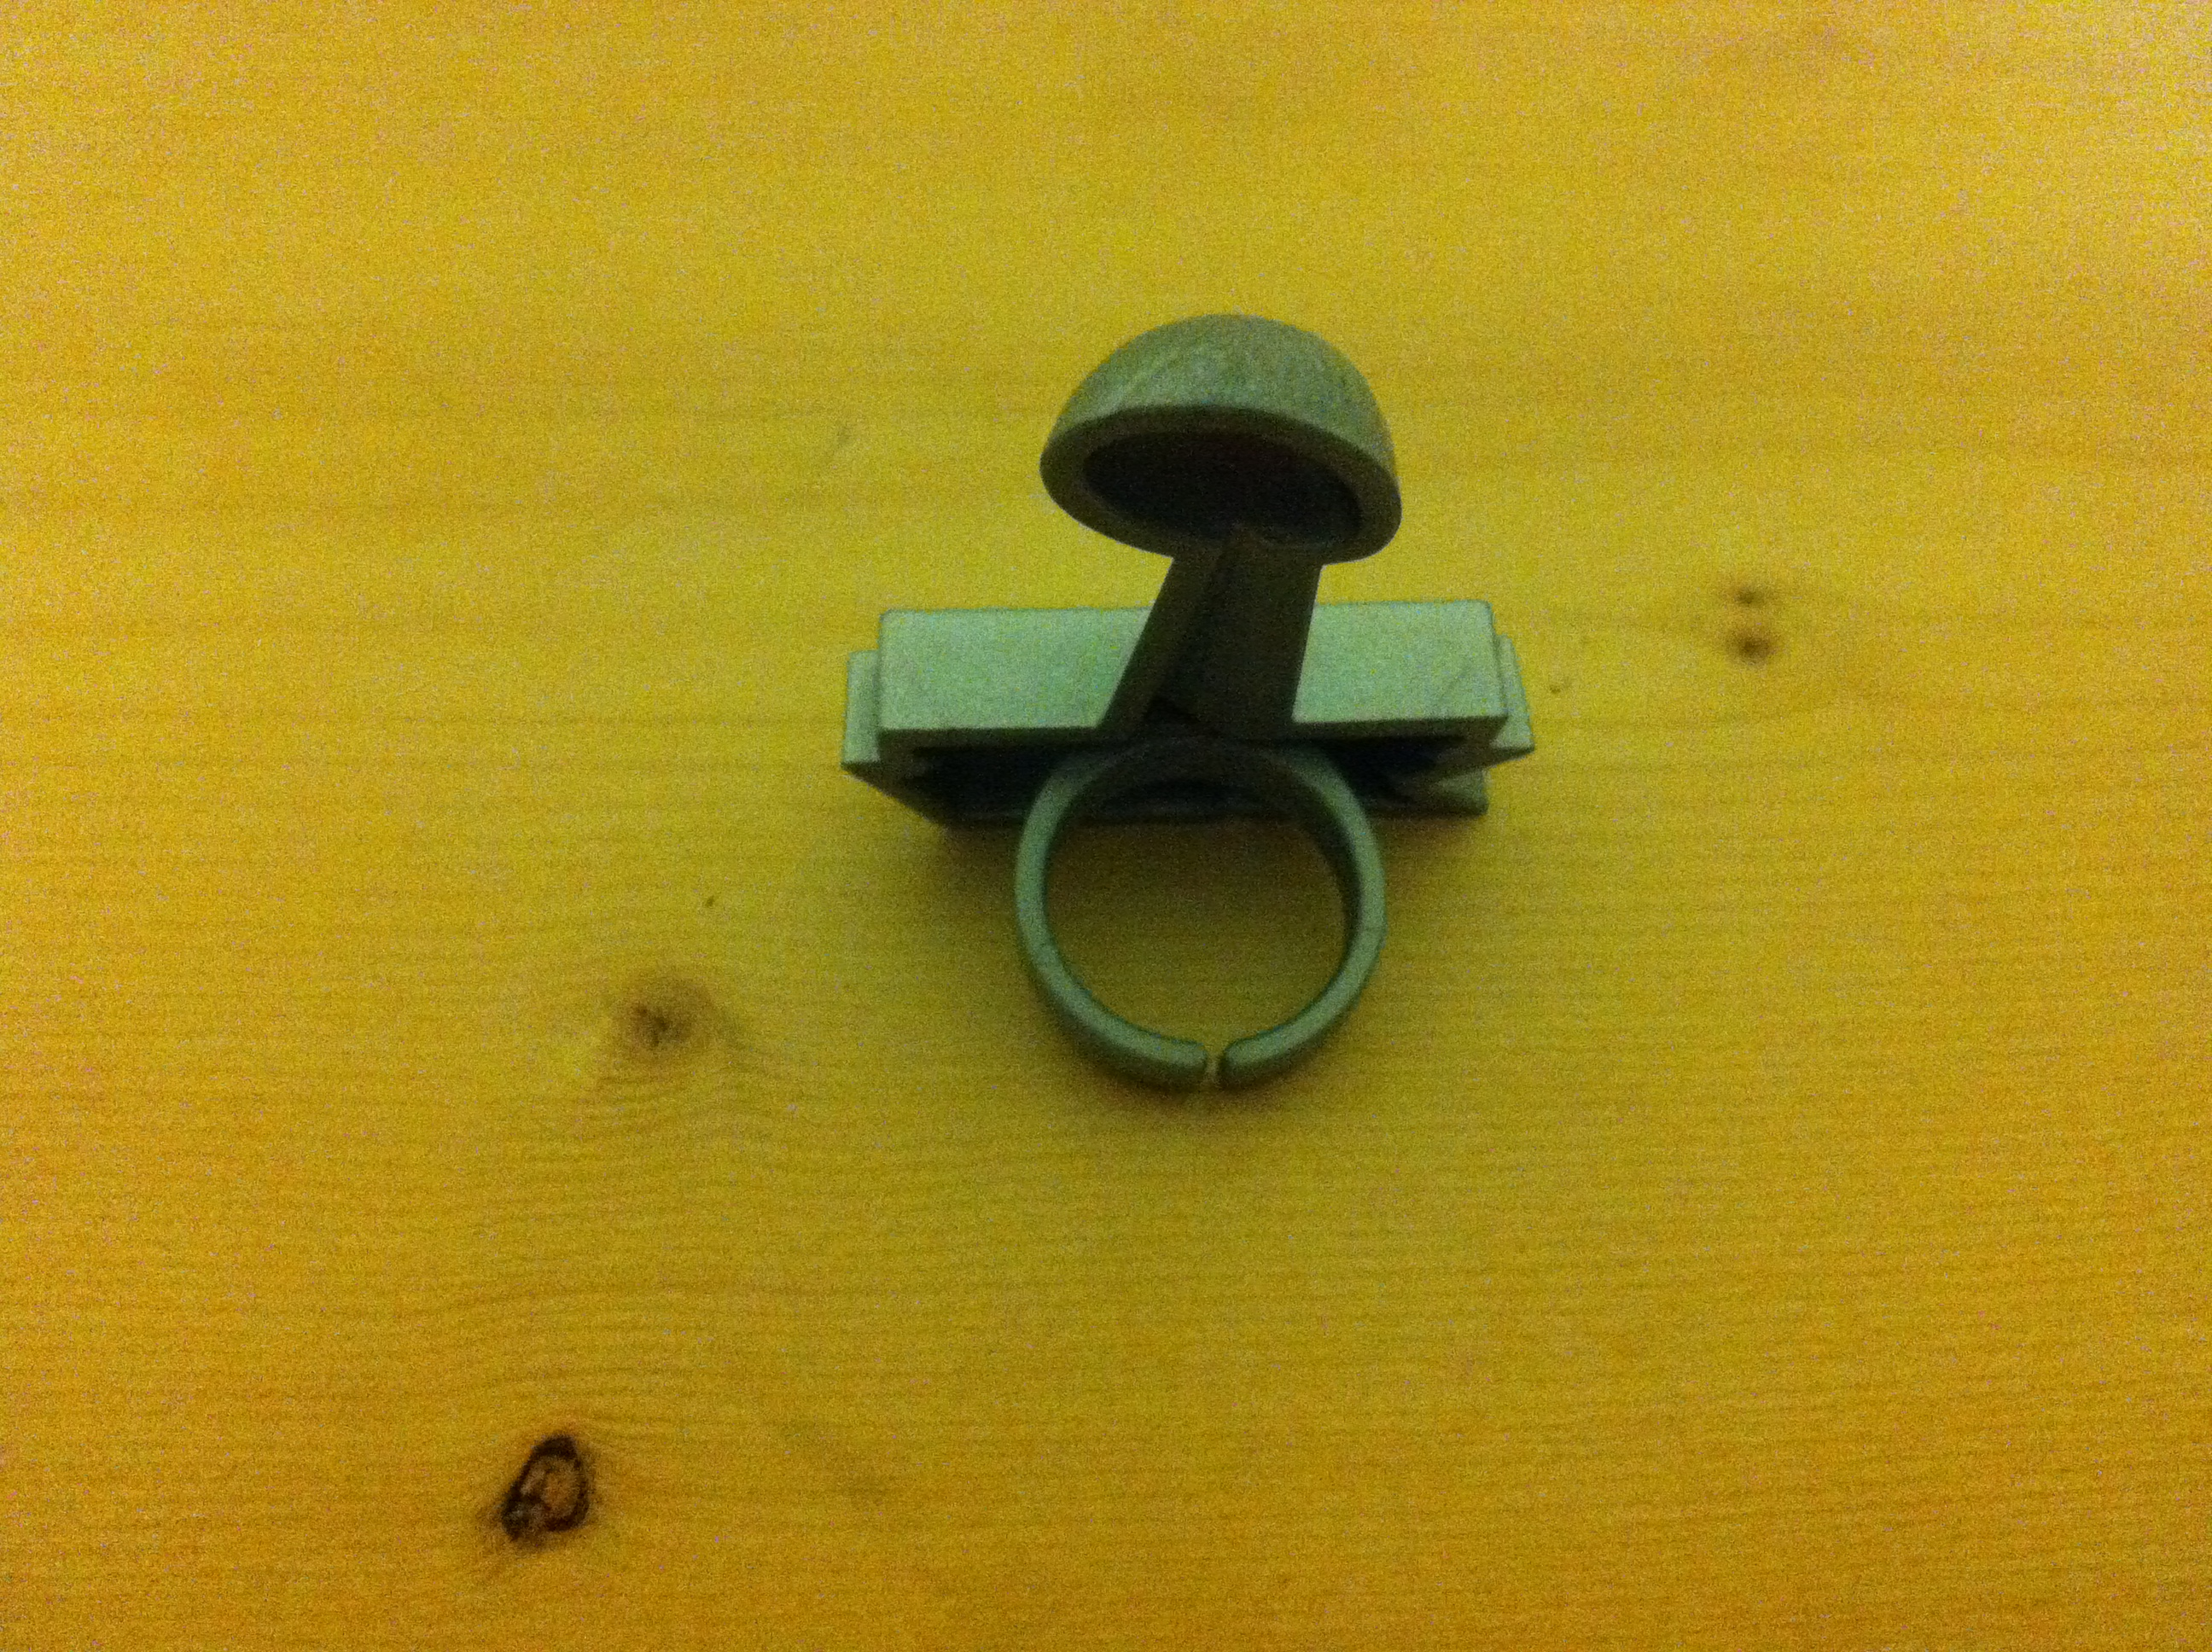
\includegraphics[width=.9\linewidth]{./ring/IMG_0370.JPG}

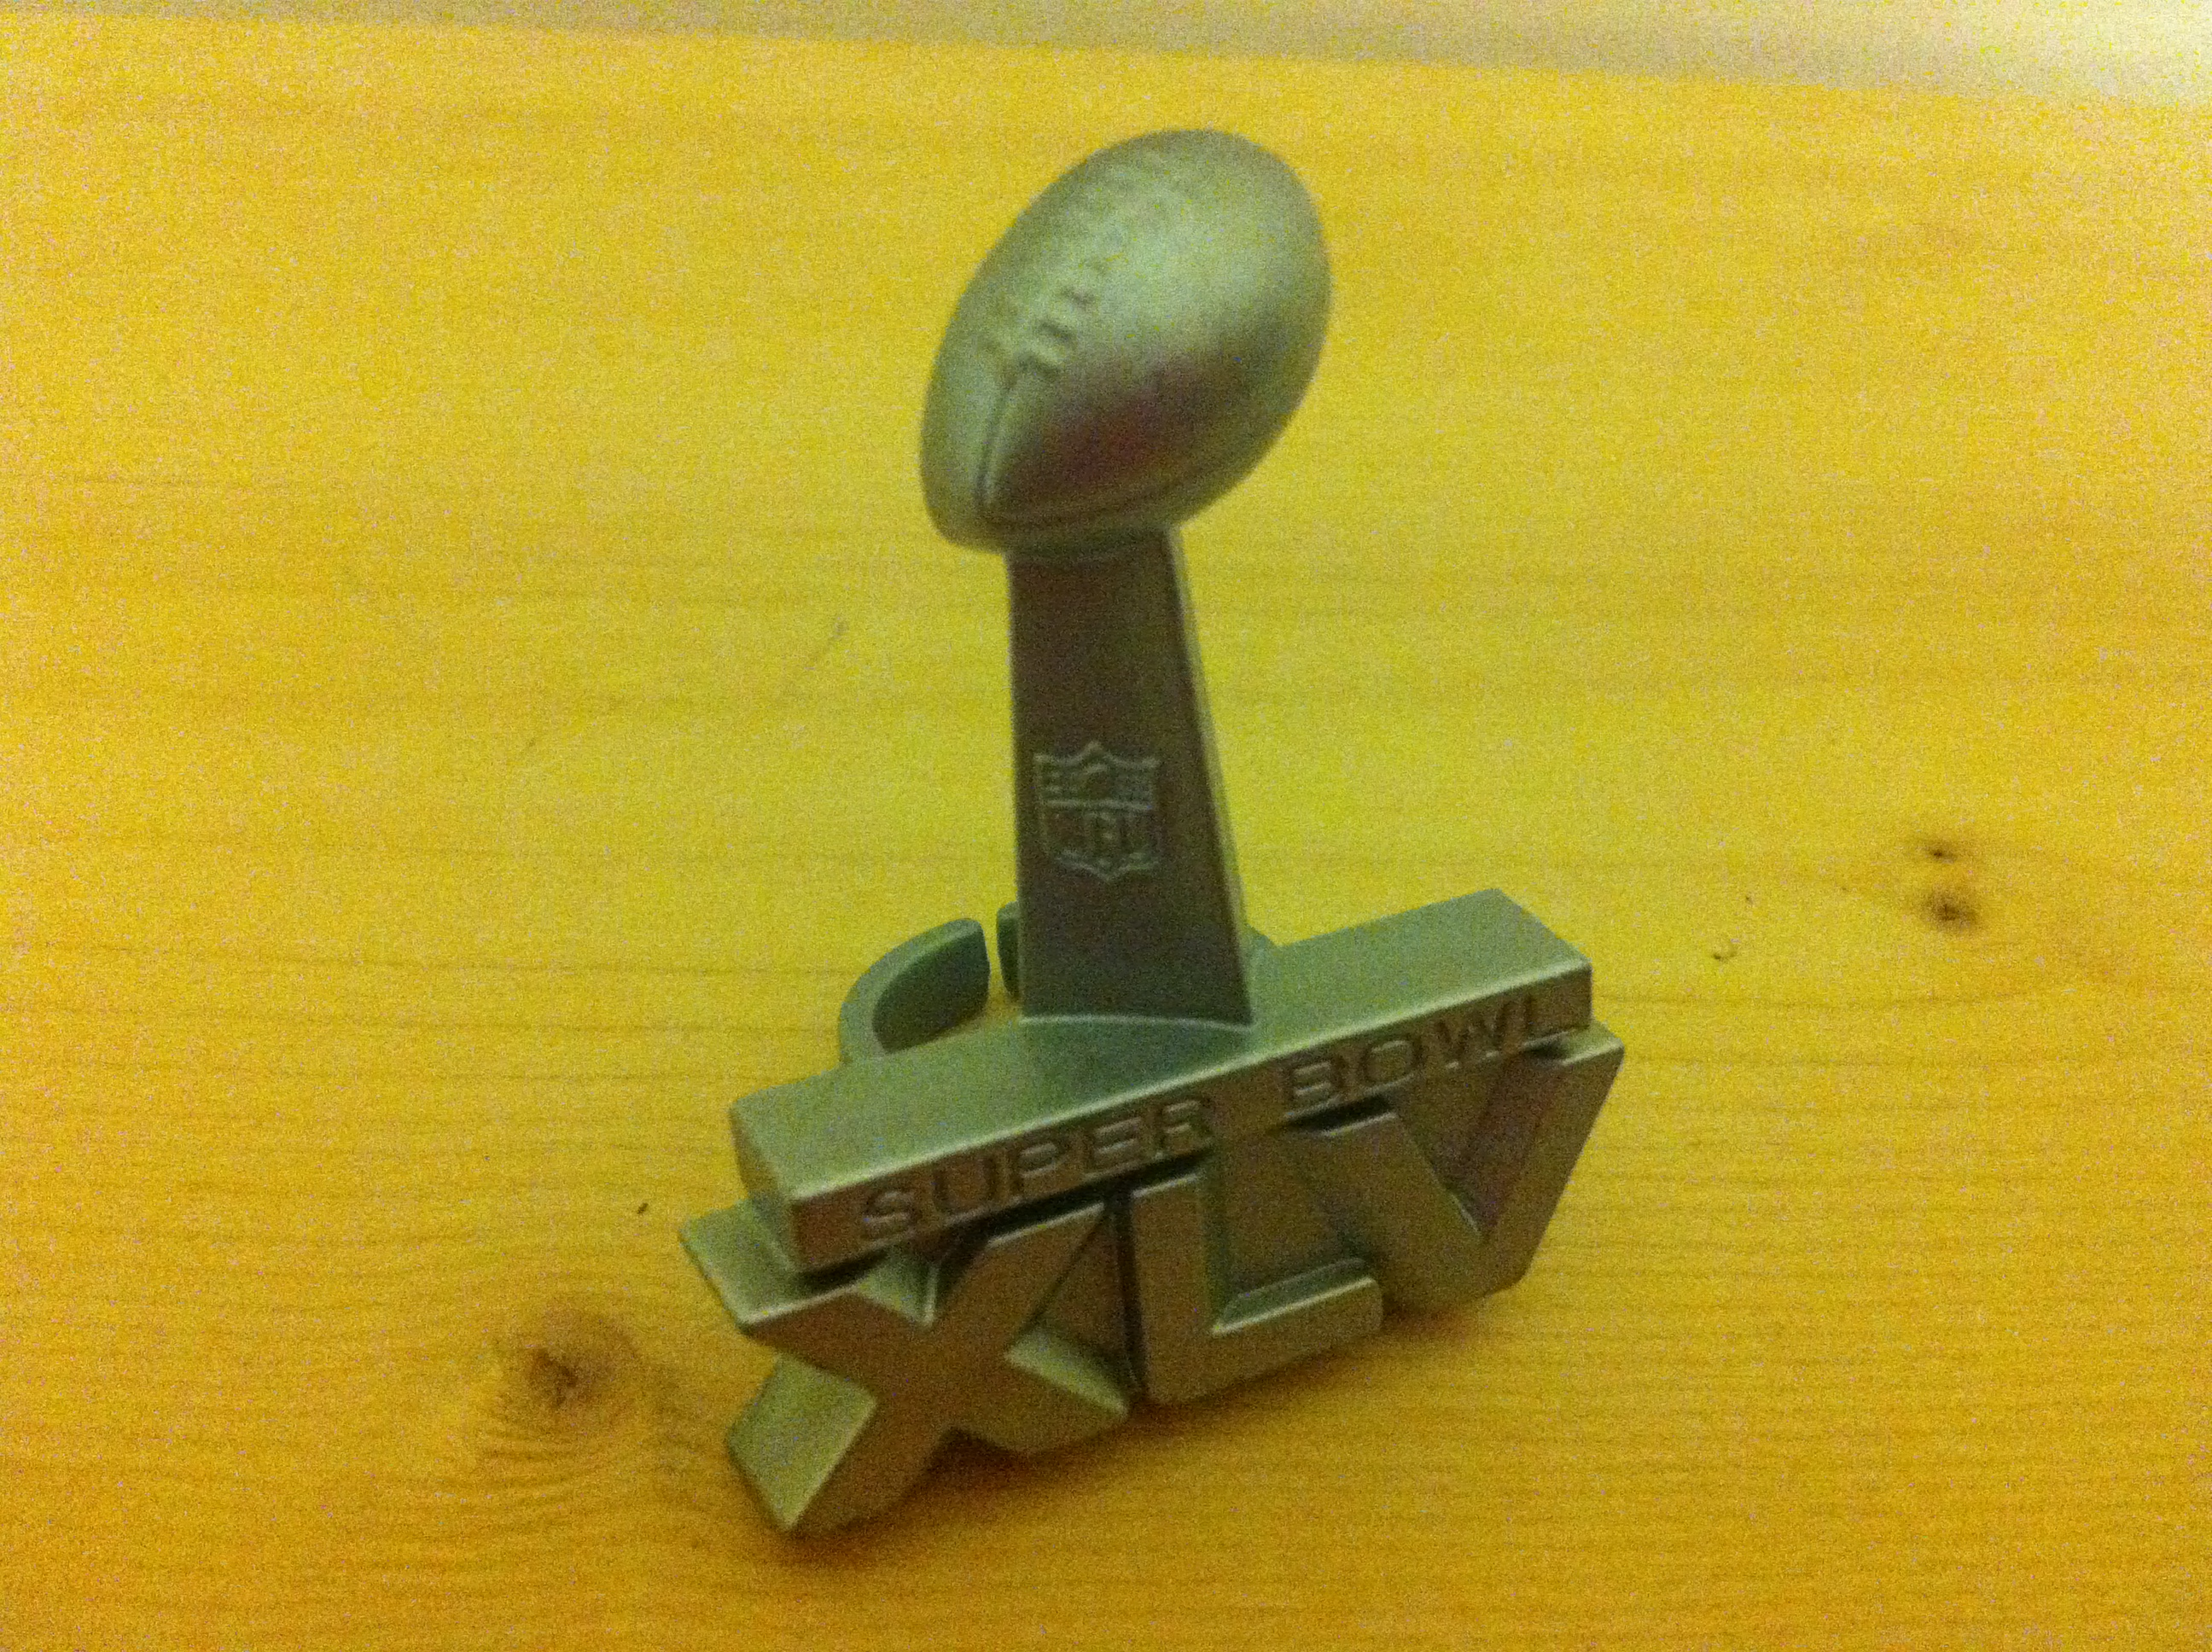
\includegraphics[width=.9\linewidth]{./ring/IMG_0371.JPG}

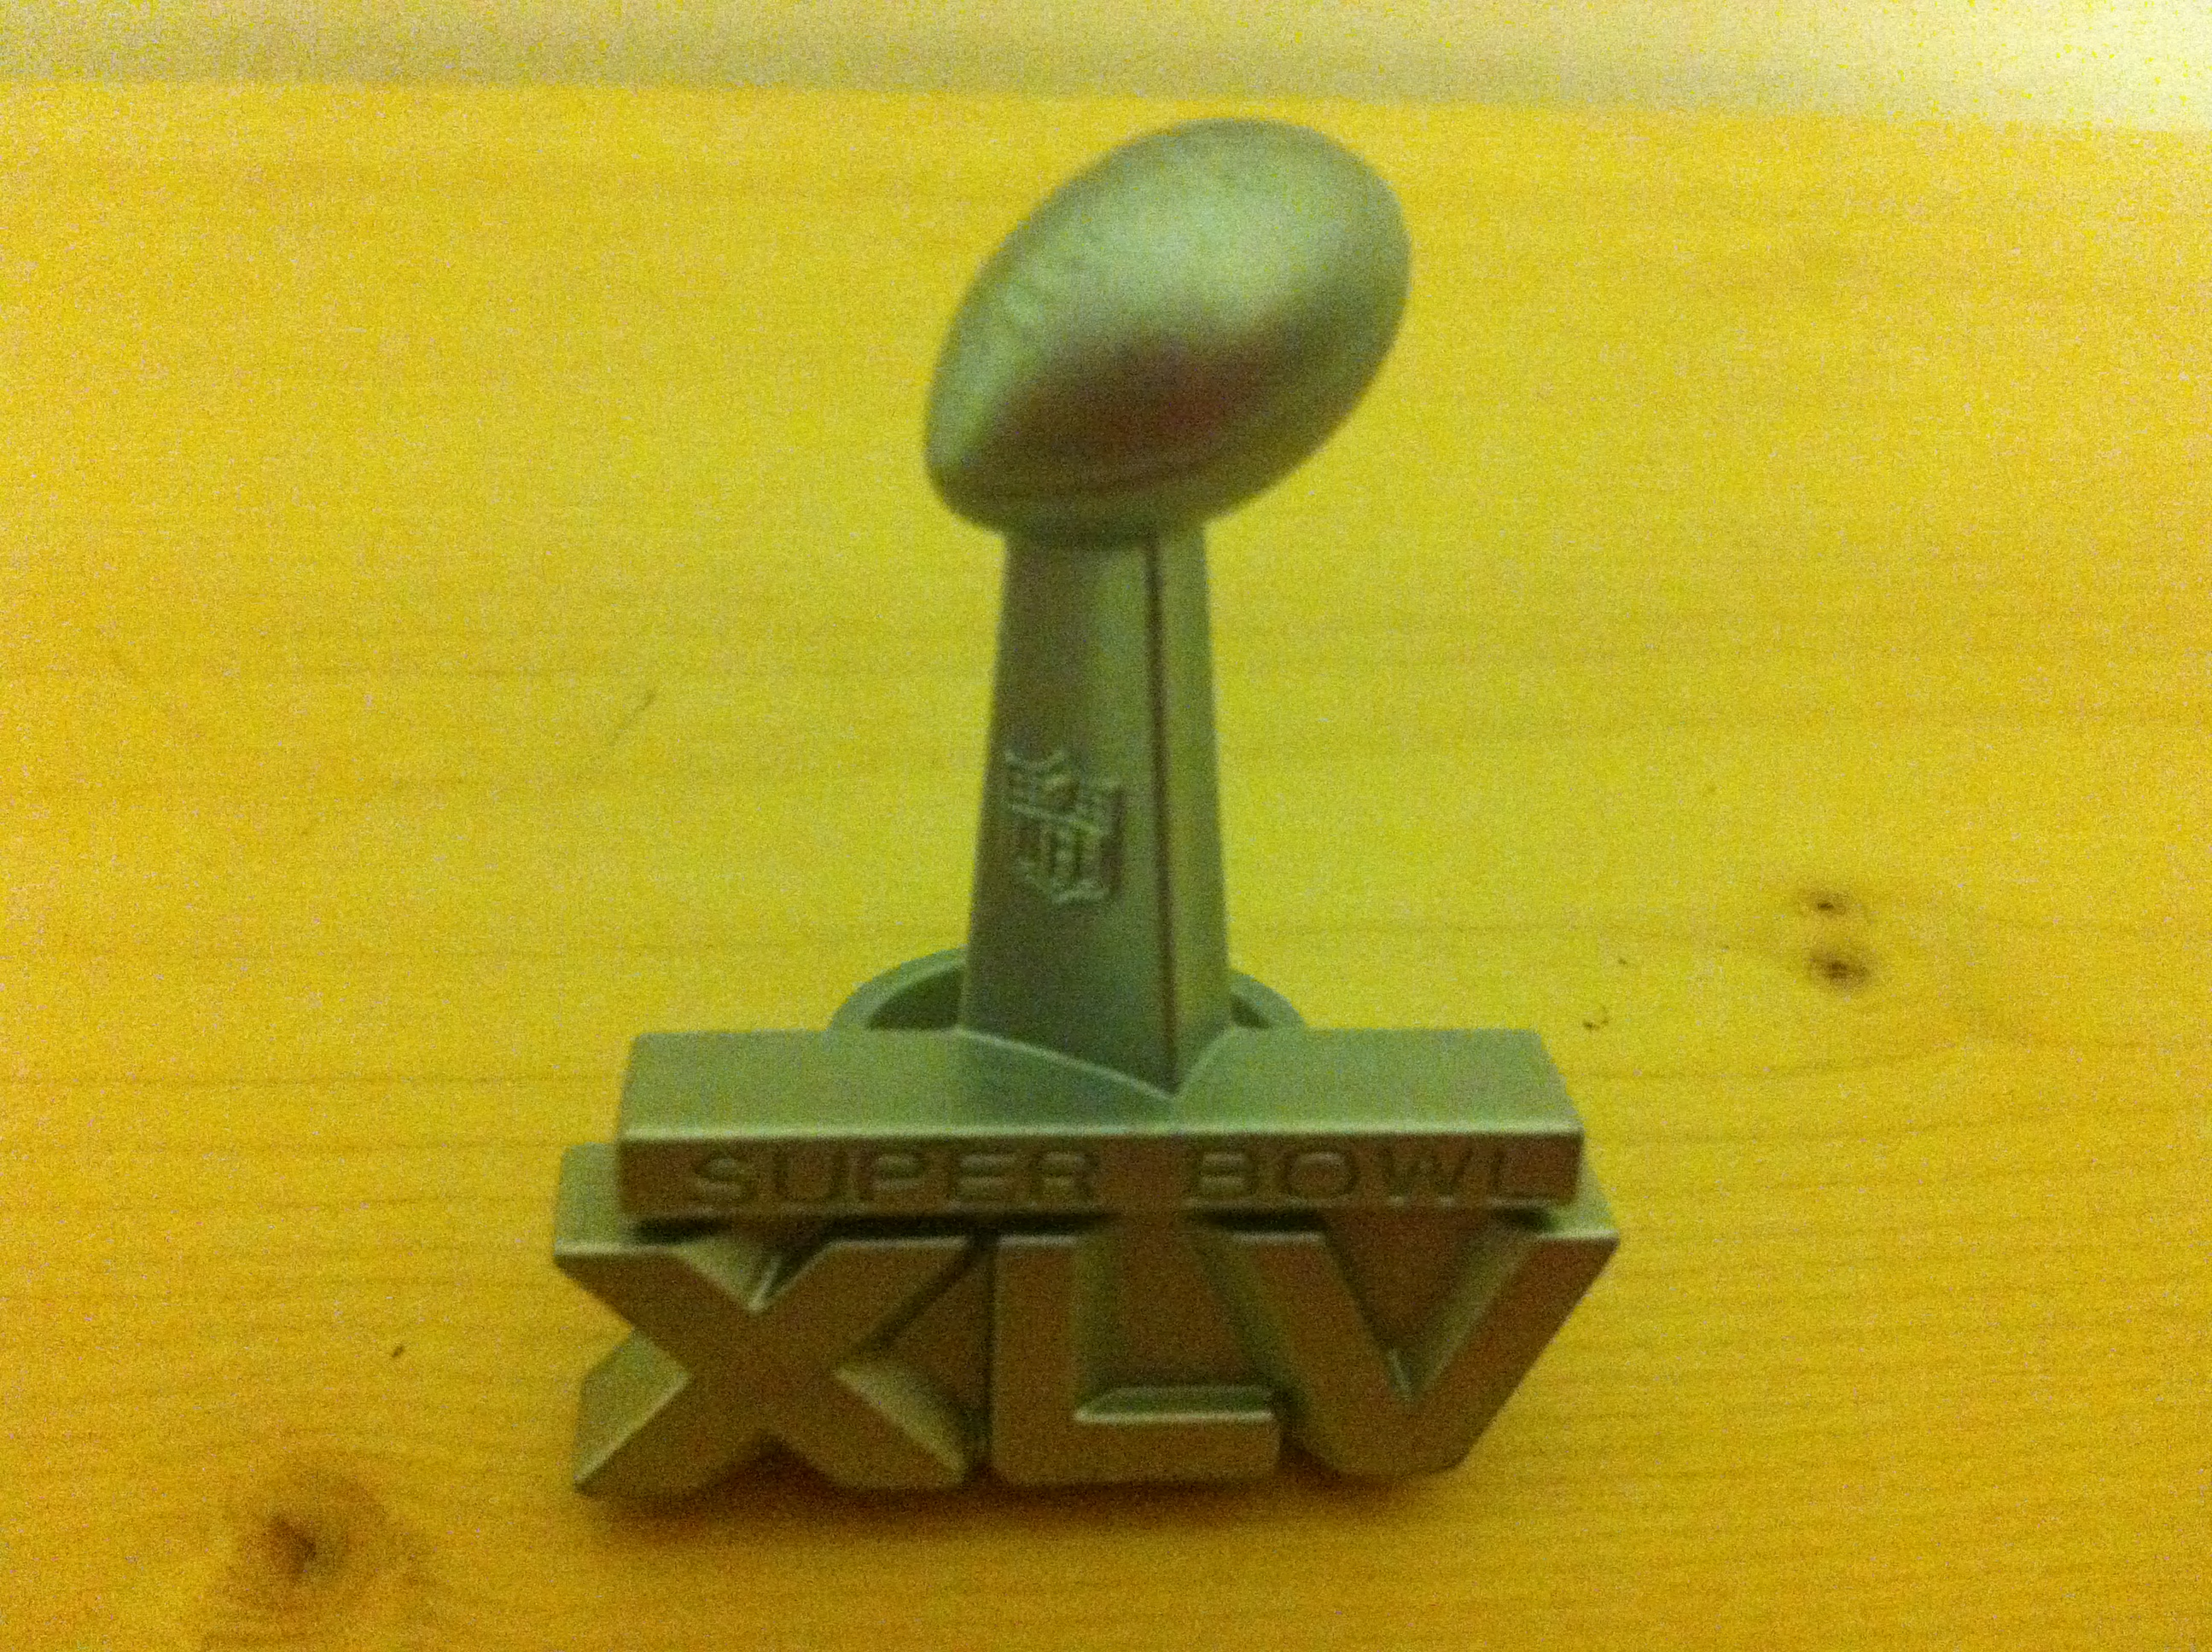
\includegraphics[width=.9\linewidth]{./ring/IMG_0372.JPG}


\includegraphics[width=.9\linewidth]{./ring/IMG_0373.JPG}


\section{About Summer Intern}
\label{sec-7}
Notes: I don't have access to my VandalMail before (like one month ago) because of password expired (I have tried to set new password, but I failed to answered the security questions with correct answers). But today when I retry to login using the google chrome remembered old password, it seems that the old password gets back (I use only one old laptop, and the password has been remembered by google chrome for months already, though I am still thinking it is more that the university ITS is playing tricks rather than my password got corrected, anyway\ldots{}.). So I will modify and paste the original emails then (even I made phone calls and got mislead, even I feel today's one day access to my email is tricks as well\ldots{}. Just too much wired happened this spring and summer!). 

I got these bunch of emails when I wrote to and asked for advisor's signature for summer intern. 

\subsection{From: (advisor\textasciitilde{}) [(advisor\textasciitilde{})@gmail.com\url{mailto:(advisor~)@gmail.com}]}
\label{sec-7-1}
Sent: Thursday, May 28, 2015 10:24 AM

To: (me\textasciitilde{}~\textasciitilde{}) ((me\textasciitilde{}~\textasciitilde{})@uxxxx.edu\url{mailto:(me~~~)@uxxxx.edu})

Subject: Re: MS CS Study Plan \_ from (me\textasciitilde{}~\textasciitilde{})

All we need to do is to fill out a "Report of Non-Thesis Requirement" form - everything else is done. If I submit this before June 12, you won't need to pay for any more credits. After June 12 you will need to register for at least 1 credit. In either case, your graduation date will be the end of summer, Aug 7.

Let me know what you want to do.

\begin{itemize}
\item (advisor\textasciitilde{})
\end{itemize}

\subsection{On Thu, May 28, 2015 at 11:52 PM, (me\textasciitilde{}~\textasciitilde{}) ((me\textasciitilde{}~\textasciitilde{})@uxxxx.edu\url{mailto:(me~~~)@uxxxx.edu}) <(me\textasciitilde{}~\textasciitilde{})@uxxxx.edu\url{mailto:(me~~~)@uxxxx.edu}> wrote:}
\label{sec-7-2}
Dr. (advisor\textasciitilde{}),

I am working on summer internship right now for these days, so I don't want you to fill out and turn in the "Report of Non-Thesis Requirement" form yet until I write to you on 6/11/2015 evening. Turn in the form by 6/12/2015 or not, it still DEPENDS.

I will continuously work on the summer intern until 6/11/2015, and I will write to you before 6/12/2015 morning 8:00am. So by 6/12/2015, if I have found any internship yet, please help me turn in the form on time so that I won't have to pay for 1 credit. But if I do find a internship working opportunity, please don't turn in the form yet, and I will work on CPT so that I can work for the summer, and I will register 1 credit for summer internship.

Please help me check the dates. If I misunderstood you or if you have any question, please let me know.

thanks.
(me\textasciitilde{}~\textasciitilde{})

\subsection{From: (advisor\textasciitilde{}) [(advisor\textasciitilde{})@gmail.com]}
\label{sec-7-3}
Sent: Sunday, May 31, 2015 10:04 PM

To: (me\textasciitilde{}~\textasciitilde{}) ((me\textasciitilde{}~\textasciitilde{})@uxxxx.edu)

Subject: Re: MS CS Study Plan \_ from (me\textasciitilde{}~\textasciitilde{})

It would be better to let me know a couple of days ahead of the 12th. I will be busy teaching a short course on June 11-12, and I will need to personally carry the form up to the Grad School in order to make it on time. So, please let me know on the 9th or 10th what you have decided. Thanks.

\begin{itemize}
\item (advisor\textasciitilde{})
\end{itemize}

\subsection{Notes}
\label{sec-7-4}
Though I got used to post email here, but bofore I wrote the followed 6/9 5:05pm email to my advisor, I did call international program office (IPO) personal, and got explained that I could always register 1 more credit if I find any summer internship, and that's the reason I felt my advisor made easy thing explained complicated and wrote the followed email to him in time and quite relaxed, and also let him know that I was working on the internship, and once I found any, I will get back to him. I didn't have the right to record the phone call, and I was naive and didn't realize the tricky and misleading part was from there. But anyway, things always happen. Tricks can win sometime, but justice always bury deep in people's heart. It was the university that I spent nine years, but it comes to the end. Let time heal all wounds\ldots{}.

\subsection{RE: MS CS Study Plan \_ from (me\textasciitilde{}~\textasciitilde{})}
\label{sec-7-5}
(me\textasciitilde{}~\textasciitilde{}) ((me\textasciitilde{}~\textasciitilde{})@uxxxx.edu)

This message was sent with High importance.

You forwarded this message on 6/22/2015 2:10 PM.

Sent:        Tuesday, June 09, 2015 5:05 PM

To:        
(advisor\textasciitilde{}) [(advisor\textasciitilde{})@gmail.com]

Dr. (advisor\textasciitilde{}), 

I checked the graduate school and made it clear for myself that I don't need any 1 more research credit, so please help me turn in the "Non-thesis requirement report form" before 6/12/2015 Friday 4:30pm. 

As for the form turn in, it could be hard copy, which would need you to carry a signed hard copy into graduate school,  I called and confirmed that you could also help scan the signed copy, and email to graduate school the electronic copy before 4:30pm this Friday. 

So please help me do that. 

If I find any intern opportunity, I will write to you so that you could help approve it for me. 

thanks in advance. 

(me\textasciitilde{}~\textasciitilde{})

\subsection{RE: MS CS Study Plan \_ from (me\textasciitilde{}~\textasciitilde{})}
\label{sec-7-6}
(me\textasciitilde{}~\textasciitilde{}) ((me\textasciitilde{}~\textasciitilde{})@uxxxx.edu)

This message was sent with High importance.

You forwarded this message on 6/22/2015 2:10 PM.

Sent:        Tuesday, June 09, 2015 5:05 PM

To:        
(advisor\textasciitilde{}) [(advisor\textasciitilde{})@gmail.com]

Dr. (advisor\textasciitilde{}), 

I checked the graduate school and made it clear for myself that I don't need any 1 more research credit, so please help me turn in the "Non-thesis requirement report form" before 6/12/2015 Friday 4:30pm. 

As for the form turn in, it could be hard copy, which would need you to carry a signed hard copy into graduate school,  I called and confirmed that you could also help scan the signed copy, and email to graduate school the electronic copy before 4:30pm this Friday. 

So please help me do that. 

If I find any intern opportunity, I will write to you so that you could help approve it for me. 

thanks in advance. 

(me\textasciitilde{}~\textasciitilde{})

\subsection{Re: CPT application Signature}
\label{sec-7-7}
(advisor\textasciitilde{}) [(advisor\textasciitilde{})@gmail.com]

You replied on 6/22/2015 10:49 PM.

Sent:        Monday, June 22, 2015 8:30 PM

To:        
(me\textasciitilde{}~\textasciitilde{}) ((me\textasciitilde{}~\textasciitilde{})@uxxxx.edu)

(Me\textasciitilde{}~\textasciitilde{}) -

As you requested, I have turned in your incompletes and your final project report, so you have graduated. Your official graduation date will be August, but you have finished. You can't take more classes unless you reapply. Besides, it is past the deadline to register for classes for summer, and I believe it is also past the time that we can add classes for summer. So unfortunately you can't register for classes at this time.

Please remember that I explained this to you, and it was your decision to have me turn in your graduation information. It is too late to change this decision now.

I wish you well in the future.

\begin{itemize}
\item (advisor)
\end{itemize}

\subsection{RE: CPT application Signature}
\label{sec-7-8}
(me\textasciitilde{}~\textasciitilde{}) ((me\textasciitilde{}~\textasciitilde{})@uxxxx.edu)

You replied on 6/26/2015 11:08 AM.

Sent:        Monday, June 22, 2015 10:49 PM

To:        
(advisor\textasciitilde{}) [(advisor\textasciitilde{})@gmail.com]

Dr. (advisor\textasciitilde{}), 

When I read your email, feels like you are the toughest advisor ever, though I had expected you to be an effective communicator and project instructor so much during spring semester. 

You kindly reminded me that "Please remember that I explained this to you, and it was your decision to have me turn in your graduation information." All the emails are attached here, and the decision I made wrote to you on 6/9/15 5:05pm were also based on the telephone call to IPO with (IPO CPT personal) for CPT. And as I stated clearly on 6/9/15 5:05pm email that "If I find any intern opportunity, I will write to you so that you could help approve it for me. " Clearly you saw I was confused and mislead, and I was still thinking about CPT for internship opportunity, but you see it though to see all these thing happen. I know xxxx is famous for potatoes, I guess maybe this university or this program should be famous for misleading international students. While still, as you strongly and toughly stated, it was my decision and mistake!

While anyway, it was an intern. if I am not able to work, I will just explain to the company then. 

I wish you well in the future, as well. 

\begin{itemize}
\item (me\textasciitilde{}~\textasciitilde{})
\end{itemize}

\subsection{RE: CPT application Signature}
\label{sec-7-9}

(me\textasciitilde{}~\textasciitilde{}) ((me\textasciitilde{}~\textasciitilde{})@uxxxx.edu)

Sent:        Friday, June 26, 2015 11:08 AM

To:        
(me\textasciitilde{}~\textasciitilde{}) ((me\textasciitilde{}~\textasciitilde{})@uxxxx.edu)

Dr. (advisor\textasciitilde{}), 

This is (Me\textasciitilde{}~\textasciitilde{}) again, your graduate student who planned to graduate this August. I just called (graduate school personal) a moment ago, and learned the fact that my spring semester csxxx is still in incomplete status, and as my graduate adviser, I will need you to help me from "work flow" to approve my application for graduation. I don't know when should be a good time for you to change csxxx incomplete to be complete, but if you could help approve my application for graduation by the end of today to meet the deadline will be great. 

If you haven any question or concern, please let me know as soon as possible. Or if you need to check some details, and feel more convenient to call me or text me instead of writing to me, my cell phone number is (555) 555-5555, and you are more than welcome to do that. 

thanks in advance, and I wish you well in the future. 

\begin{itemize}
\item (me\textasciitilde{}~\textasciitilde{})
\end{itemize}

\subsection{one day only access to the old email? fdfjdfdkfjdlklsdfjdoisfj}
\label{sec-7-10}

Important Notice - University of xxxx password expiration - account huanxxx

ITS Help Desk [helpdesk@uxxxx.edu]
Sent:        Monday, August 17, 2015 7:00 AM
To:        
(me\textasciitilde{}~\textasciitilde{}) ((me\textasciitilde{}~\textasciitilde{})@uxxxx.edu)


University of xxxx          !                   Password Expiration Notice         

The password for your University of xxxx account "huanxxx" will expire and be unusable within the next two weeks.

Your huanxxx password will expire in:
1 Day

When will my password expire?

Your huanxxx password will expire on August 18 at 8:37 PM. After your password has expired it cannot be used for any services except the Account Management page at help.uxxxx.edu.

How do I change my password?
Visit the Account Management page at help.uxxxx.edu
Sign-in with your existing password (even if it has expired)
Select the "Change Passwords" menu item
Instructions for changing a forgotten password are available here:
\url{http://www.uxxxx.edu/its/Self-Help/Accounts-and-Passwords/Reset-your-NetID-Password}

How do I reset my password if I don't remember it?

If you have setup a "Security Profile," consisting of 3 security questions and 1 verified phone or email contact, you may use the password reset option on the help.uxxxx.edu site.

Instructions for setting up a Security Profile are available here:
\url{http://www.uxxxx.edu/its/Self-Help/Accounts-and-Passwords/Setting-up-your-Security-Profile}

Quick tips for Password Safety
Use a long, memorable password at least 15 characters long.
Use a unique password for each of your accounts.
Never use your University of xxxx password on another site.
Never share your password, not even with the ITS Help Desk.
Only enter your UI password on "uxxxx.edu" websites.
How do I identify University of xxxx websites?
Look for "uxxxx.edu" in your web browser.
Look for the green lock with "University of xxxx [US]".

Who do I contact for technical issues?

If you have any questions, or have problems changing your password, please visit the ITS Help Desk in the xxxx place/place room xxx with a photo id. The ITS Help Desk can also be reached by phone at 555-555-HELP (4357) or by e-mail at helpdesk@uxxxx.edu.

\textbf{Goodbye, uxxxx\textasciitilde{}~\textasciitilde{}!}
% Emacs 24.3.1 (Org mode 8.2.7c)
\end{document}